\documentclass[11pt,spanish]{article}

% Paquetes
\usepackage{amstext}
\usepackage{amssymb}
\usepackage{amsmath}
\usepackage{babel}
    \addto\shorthandsspanish{\spanishdeactivate{~<>}}
    \decimalpoint
\usepackage[style=iso]{datetime2}
\usepackage{fancyhdr}
\usepackage{float}
\usepackage[T1]{fontenc}
\usepackage[a4paper]{geometry}
    \geometry{verbose,tmargin=3cm,bmargin=2cm,lmargin=2.5cm,rmargin=2.5cm}
\usepackage{graphicx}
\usepackage{hyperref}
\usepackage[utf8]{inputenc}
\usepackage{lastpage}
\usepackage{mathptmx}
\usepackage{tasks}
\usepackage{units}
\usepackage{siunitx}

% dibujos 

\usepackage{tikz}
\usepackage{tikz-dimline}
\usetikzlibrary{calc}
% \usetikzlibrary{math}
\usetikzlibrary{arrows.meta}
\usetikzlibrary{snakes}
\usetikzlibrary{decorations}
\usetikzlibrary{decorations.pathmorphing}
\usetikzlibrary{patterns}

% tipo de fuente 
\usepackage{lmodern}

\pagestyle{fancy}
\lfoot{\small DF, FCEyN, UBA}
\cfoot{\tiny Actualizado el {\today} a las {\DTMcurrenttime}}
\rfoot{\small Pág. {\thepage} de \pageref{LastPage}}

\begin{document}

% Título
    \begin{center}
   \textsc{\large Física 2 (Física) -- Cátedra Diego Arbó}
    \par\end{center}{\large \par}
    
    \begin{center}
    \textsc{\large Primer Cuatrimestre de 2025}
    \par\end{center}{\large \par}
    
    \begin{center}
    \textsc{\large Guía 5: Interfaces Entre Diferentes Medios}
    \par\end{center}{\large \par}

% Comienzo 
\begin{enumerate}

\section*{Reflexión y transmisión en cuerdas}


% Ejercicio 1

    \item Se tienen dos cuerdas semi--infinitas, de densidades lineales
    $\mu_{1}$ y $\mu_{2}$, unidas en un punto. El sistema está sometido a una
    tensión constante $T_0$. Sobre la primera cuerda (la de densidad $\mu_{1}$)
    incide una onda de la forma:
    $\psi_\text{I}(x,t)=A_\text{I}\cos\left(k_{1}x-\omega t\right)$. Se
    conocen: $\mu_{1}$, $\mu_{2}$, $T$, $\omega$ y $A_\text{I}$.

    \begin{figure}[H]
    \centering
        \begin{tikzpicture}[scale= 1]
    		\draw [ultra thick, dashed] (-3,0) -- (-2,0);
    		\draw [ultra thick] (-2,0) -- (0,0) node [near start, above] {\(\mu_{1} \)};
    		\draw [thin] (0,0) -- (2,0) node [near end, above] {\(\mu_{2} \)}; % node [midway, above] {\(\lambda_{m2} \)};
    		\draw [thin, dashed] (2,0) -- (3,0);
    	\end{tikzpicture}
    \end{figure}

    \begin{enumerate}
        \item Calcule $k_{1}$ y $k_{2}$, es decir, los números de onda de cada
        lado de la unión.
        \item Plantee la solución más general para $\psi(x,t)$ de cada lado de
        la unión.
        \item ¿Qué condiciones deben verificarse en el punto de unión de las
        cuerdas?
        \item Usando (b) y (c), calcule la perturbación $\psi(x,t)$ en cada una
        de las cuerdas. 
        \item Determine coeficientes de reflexión, $R$, y transmisión, $T$.
        ¿Qué sucede en el caso \(\mu_{2} \rightarrow \infty\)? ¿Y si
        \(\mu_{1} \to \mu_{2}\)? 
    \end{enumerate}

% Ejercicio 2

    \item La cuerda de la izquierda, de densidad lineal \(\mu_1\) y largo \(L\),
    se encuentra fija en su extremo izquierdo a la pared, y en su extremo
    derecho a otra cuerda semi-infinita de densidad \(\mu_2\). Todo el
    sistema se encuentra sometido a la misma tensión \(T_0\). Suponga que por
    la cuerda de densidad \(\mu_2\) incide la onda armónica
    \(\psi_\text{I}(x,t) = A_\text{I} \mathrm{e}^{i (\omega t + k_2 x) }\).

    \begin{figure}[H]
    \centering
    	\begin{tikzpicture}[scale= 1]
    		\draw (-2,-1) -- (-2,1); % pared vertical
    		\fill [pattern = north east lines] (-2.25,-1) rectangle (-2,1);
    		\draw [ultra thick] (-2,0) -- (0,0) node [midway, above] {\(\mu_1 \)};
    		\draw [thin] (0,0) -- (3,0) node [midway, above] {\(\mu_2 \)};
    		\dimline [extension start length= -0.2, extension end length = -0.2] {(-2,-0.4)}{(0,-0.4)}{\(L\)}; 
    		\draw [thin, dashed] (3,0) -- (4,0);
    	\end{tikzpicture}
    \end{figure}

    \begin{enumerate}
    	\item Imponga las condiciones de contorno apropiadas y determine
        \(\psi(x,t)\) en cada sección del sistema.
    	\item Halle los valores de \(L\) para los cuales hay un nodo de
        desplazamiento en la unión de las cuerdas.
    \end{enumerate}

% Ejercicio 3

    \item Una cuerda de densidad lineal \(\mu\) sometida a una tensión
    \(T_0\) tiene en su centro, \(x= 0\), un pequeño nudo de masa \(M\).
    Cuando una onda \(\psi_i(x,t) = A_i \mathrm{e}^{i ( k x - \omega t ) }\)
    incide desde el infinito, el nudo causa que parte de la onda incidente sea
    reflejada, y otra parte transmitida.
    
    \begin{figure}[H]
    \centering
    	\begin{tikzpicture}[scale= 1]
    		\draw [thick, dashed] (-3,0) -- (-2,0);
    		\draw [thick] (-2,0) -- (0,0) node [near start, above] {\(\mu \)};
    		% \draw [thick] (-2,0) -- (2,0); % node [midway, above] {\(\lambda_{m2} \)};
    		\draw [thick] (0,0) -- (2,0) node [near end, above] {\(\mu \)};
    		\draw [thick,dashed] (2,0) -- (3,0);
    		\shade [ball color=black!80] (0,0) circle(0.25) node [] {\color{white} $M$};
    	\end{tikzpicture}
    \end{figure}
    
    \begin{enumerate}
    	\item Plantee la solución más general para la onda \(\psi (x,t)\) a
        cada lado del nudo.
    	\item ¿Qué condiciones de empalme deben verificarse en el nudo?
    	\item Demuestre que una condición le permite definir que
        \(A_\text{I} + A_\text{R} = A_\text{T}\) y que la otra implica que
        \(A_\text{I} - A_\text{R} = (1 + i \frac{M \omega^2}{k T} )A_\text{T}\),
        siendo $A_\text{I}$, $A_\text{R}$ y $A_\text{T}$ las amplitudes
        complejas para las ondas incidente, reflejada y transmitida,
        respectivamente.
    \end{enumerate}


\section*{Reflexión y transmisión en ondas acústicas}

% Ejercicio 4

    \item Se tienen dos caños semi--infinitos de distinta sección y unidos, como
    se muestra en la figura. Una onda acústica de la forma
    $\delta p_\text{I}(x,t)=A_\text{I}\cos\left(k_{1}x-\omega t\right)$ incide
    desde el primer caño hacia $x>0$. Hallar las amplitudes de presión
    $\delta \rho$ y desplazamiento $\psi$ de las ondas reflejadas y transmitidas.

    \begin{figure}[H]
        \centering{}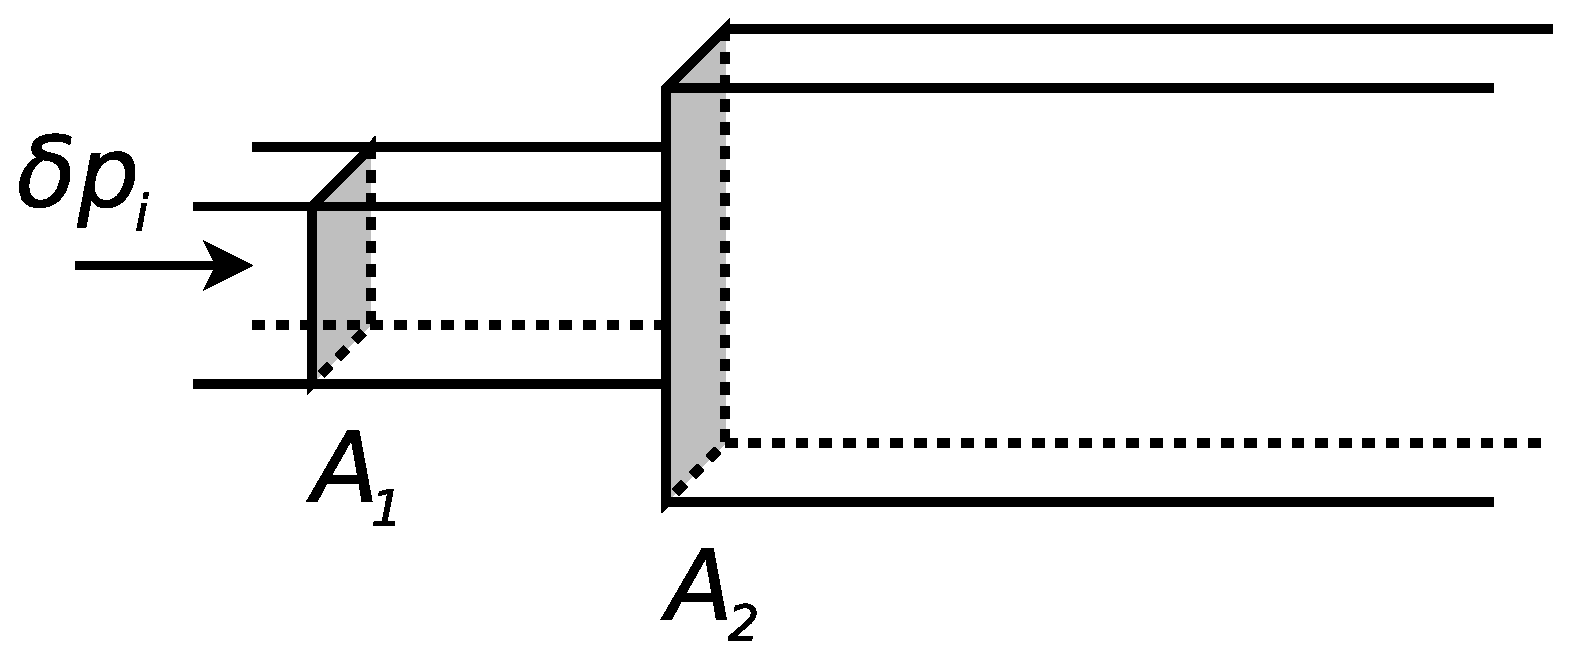
\includegraphics[clip,scale=0.25]{figs/ej2-10}
    \end{figure}

    \begin{description}
        \item [{Datos:}] $A_{1}$, $A_{2}$, presión media $P_{0}$, densidad media
        $\rho_{0}$, $v_\text{s}$, $\omega$, $A_{i}$. Suponer despreciables
        los efectos de la viscosidad. 
    \end{description}

% Ejercicio 5

    \item Considere la siguiente configuración: 
    \begin{figure}[H]
        \centering{}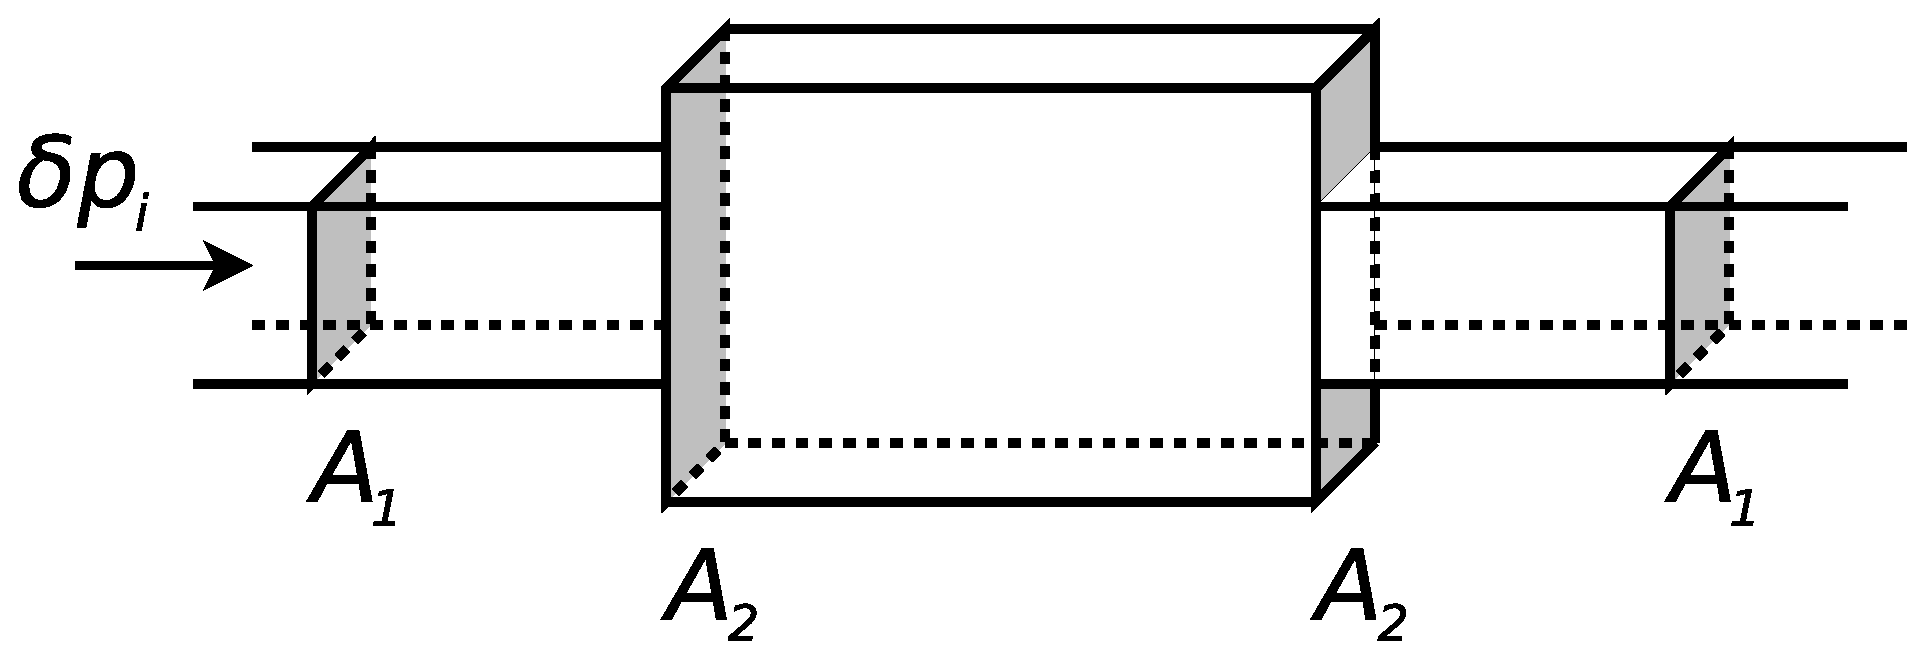
\includegraphics[clip,scale=0.25]{figs/ej2-11}
    \end{figure}
    Suponga que desde la izquierda incide una onda cuya expresión es la misma
    del problema anterior (las secciones y el resto de los datos son los mismos
    también). Hallar $\delta p(x,t)$ y $\psi(x,t)$ en cada tramo.

% Ejercicio 6

    \item Se tiene una interfase plana e infinita entre aire y agua (ver figura).
    \begin{figure}[H]
        \centering{}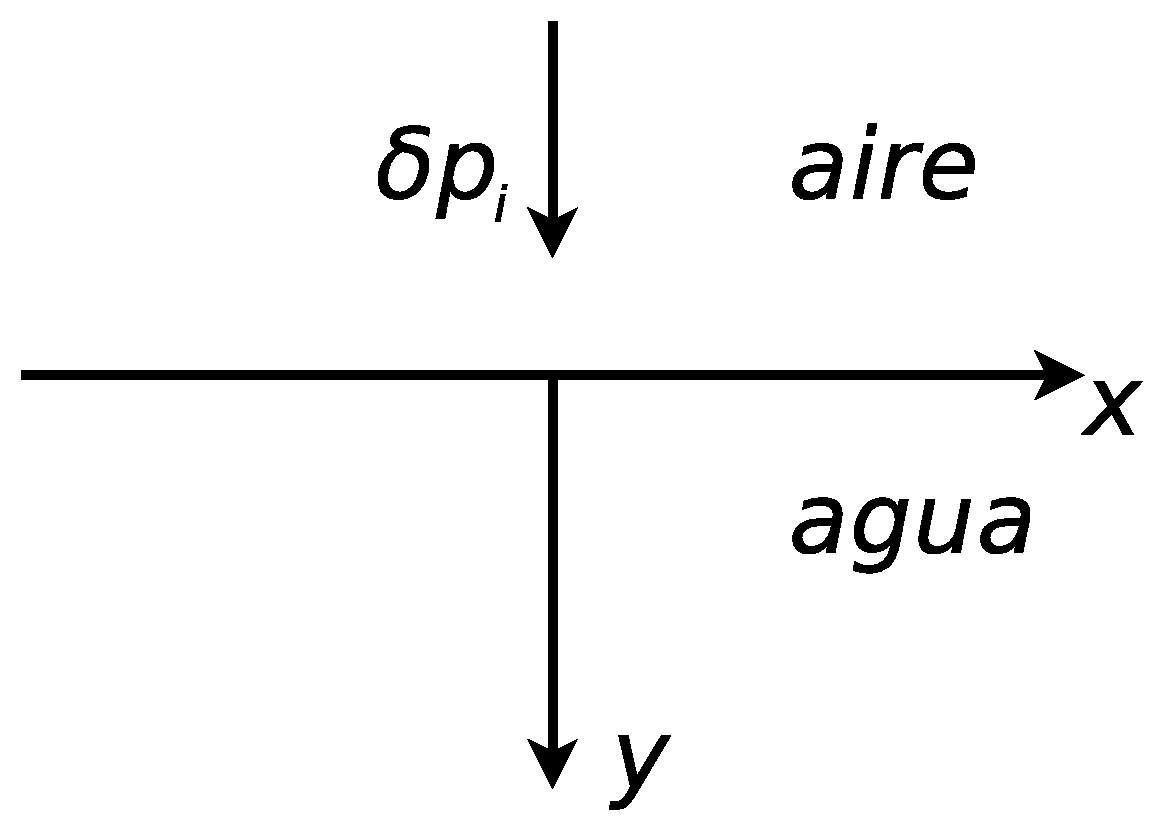
\includegraphics[clip,scale=0.25]{figs/ej2-12}
    \end{figure}
    Desde el aire incide una onda acústica plana cuya dirección de propagación
    es normal a la interfase; se escribe
    $\delta p_\text{I}(y,t)=A_\text{I}\cos\left(k_\text{aire}y-\omega t\right)$.
    Hallar las ondas reflejadas y transmitidas $\delta p_\text{R}(y,t)$ y
    $\delta p_\text{T}(y,t)$.

% Ejercicio 7

    \item Considere la ecuación de ondas clásica en tres dimensiones.

    \begin{enumerate}
        \item Demuestre que la función
        $\psi(\mathbf{r},t)=Ae^{i(\mathbf{k}\cdot\mathbf{r}\pm\omega t)}$,
        con $\mathbf{k}=k_{x}\hat{x}+k_{y}\hat{y}+k_{z}\hat{z}$ un vector
        constante y $\mathbf{r}=x\hat{x}+y\hat{y}+z\hat{z}$, es solución de la
        ecuación de ondas tridimensional. \textbf{Sugerencia:} exprese el
        laplaciano en coordenadas cartesianas.

        \item Analice el significado físico de $\psi(\mathbf{r},t)$. ¿Cómo son
        los frentes de onda? ¿Cuál es la relación entre el vector $\mathbf{k}$
        y los frentes de onda? ¿Hacia dónde se desplazan los frentes de onda
        al transcurrir $t$? ¿A qué velocidad?

        \item Rehaga el problema anterior suponiendo que la onda incidente
        (desde el aire) forma un ángulo $\theta$ con la normal a la interfase
        (ver figura).
        \begin{figure}[H]
            \centering{}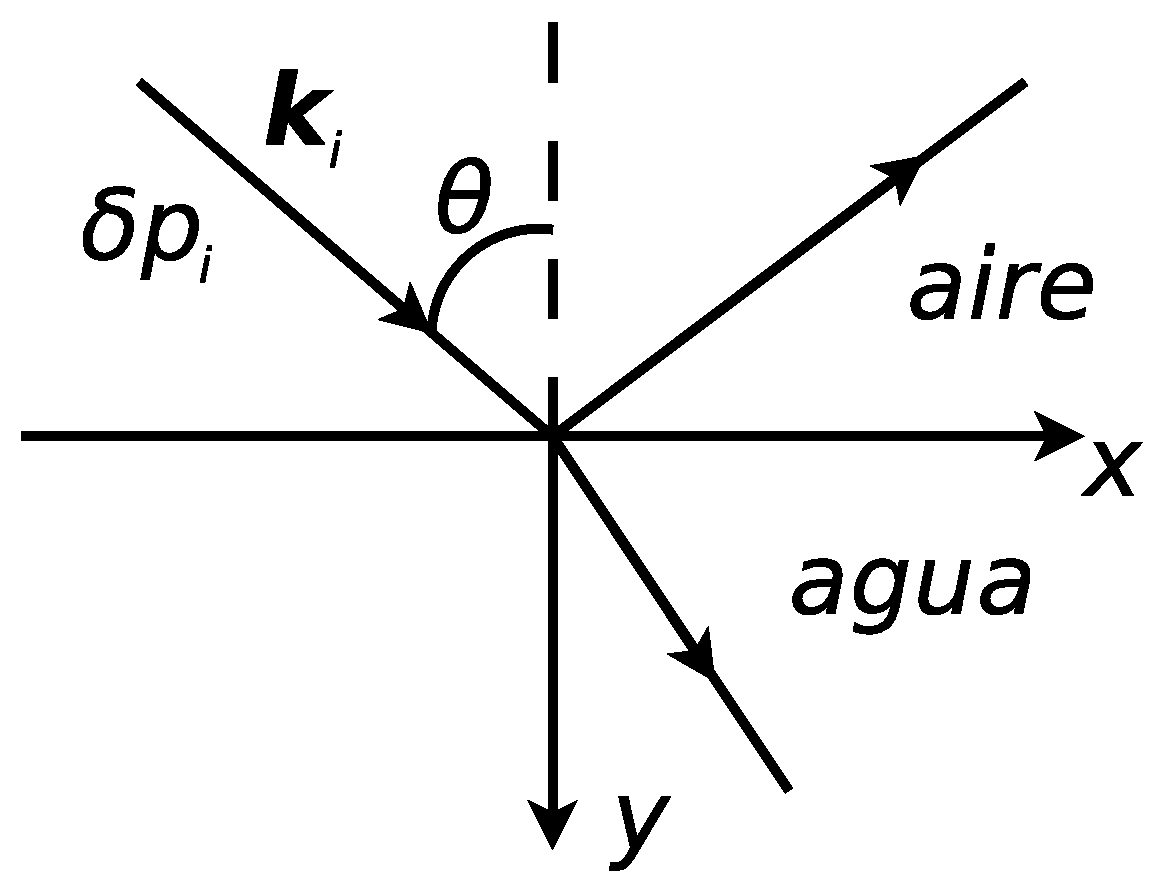
\includegraphics[clip,scale=0.25]{figs/ej2-13}
        \end{figure}
        Por lo tanto la onda de presión incidente se escribe, si usamos notación
        compleja:
        $\delta p_\text{I}(\mathbf{r},t)=A_\text{I}e^{i(\mathbf{k}_\text{I}\cdot\mathbf{r}-\omega t)}$,
        siendo
        $\mathbf{k}_\text{I}=\frac{\omega}{v_\text{s}}\left(\sin\theta\hat{x}+\cos\theta\hat{y}\right)$,
        con $v_\text{s}$ la velocidad del sonido en aire.
        Hallar la onda reflejada
        $\delta p_\text{R}(\mathbf{r},t)=A_\text{R}e^{i(\mathbf{k}_\text{R}\cdot\mathbf{r}-\omega t)}$
        y la transmitida $\delta p_\text{T}(\mathbf{r},t)=A_\text{T}e^{i(\mathbf{k}_\text{T}\cdot\mathbf{r}-\omega t)}$.
    \end{enumerate}

\section*{Regímenes de propagación dispersivo y reactivo}

% Ejercicio 8

    \item Considere un arreglo lineal de péndulos acoplados excitados cuyo
    extremo inferior está en $z=0$ y unidos a una pared rígida en $z=L$, como
    se muestra en la figura.

    \begin{figure}[H]
        \centering{}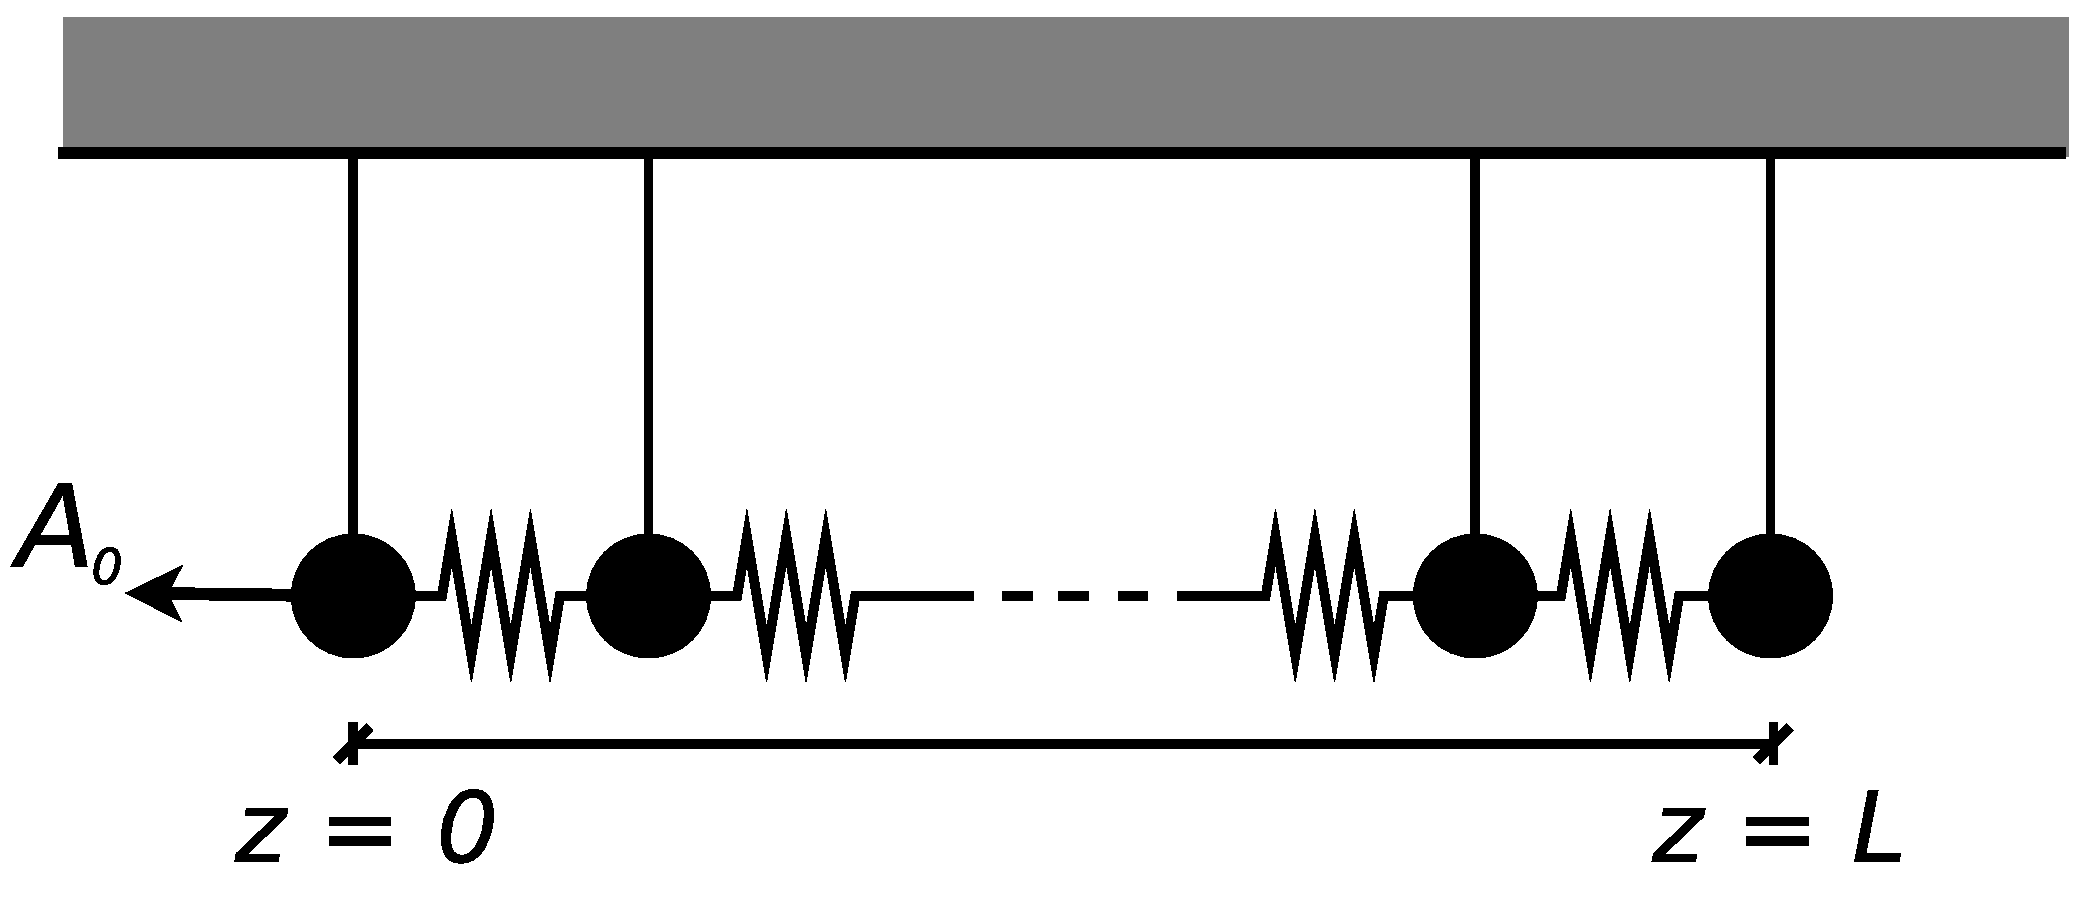
\includegraphics[clip,scale=0.25]{figs/ej1-15}
    \end{figure}

    Se aplica una fuerza externa en función del tiempo a la primera masa
    ($z=0$), de forma tal que se conoce su amplitud
    $\psi(0,t)=A_{0}\cos(\Omega t)$. Halle el movimiento estacionario del
    sistema y discuta las hipótesis que hace. Compare con el caso de extremo
    derecho fijo a una pared (o sea: agregando un resorte a la derecha de la
    última masa y uniéndolo a la pared).

    \textbf{Sugerencia:} Use la aproximación continua (mediante la ecuación de
    Klein-Gordon) para simplificar los cálculos.

% Ejercicio 9

    \item Considere un sistema de péndulos acoplados con un cambio brusco en
    $\omega_{0}^{2}$ en $z=L$, según se esquematiza en la figura. Halle el
    movimiento estacionario del sistema y discuta las hipótesis que hace.

    \begin{figure}[H]
        \centering{}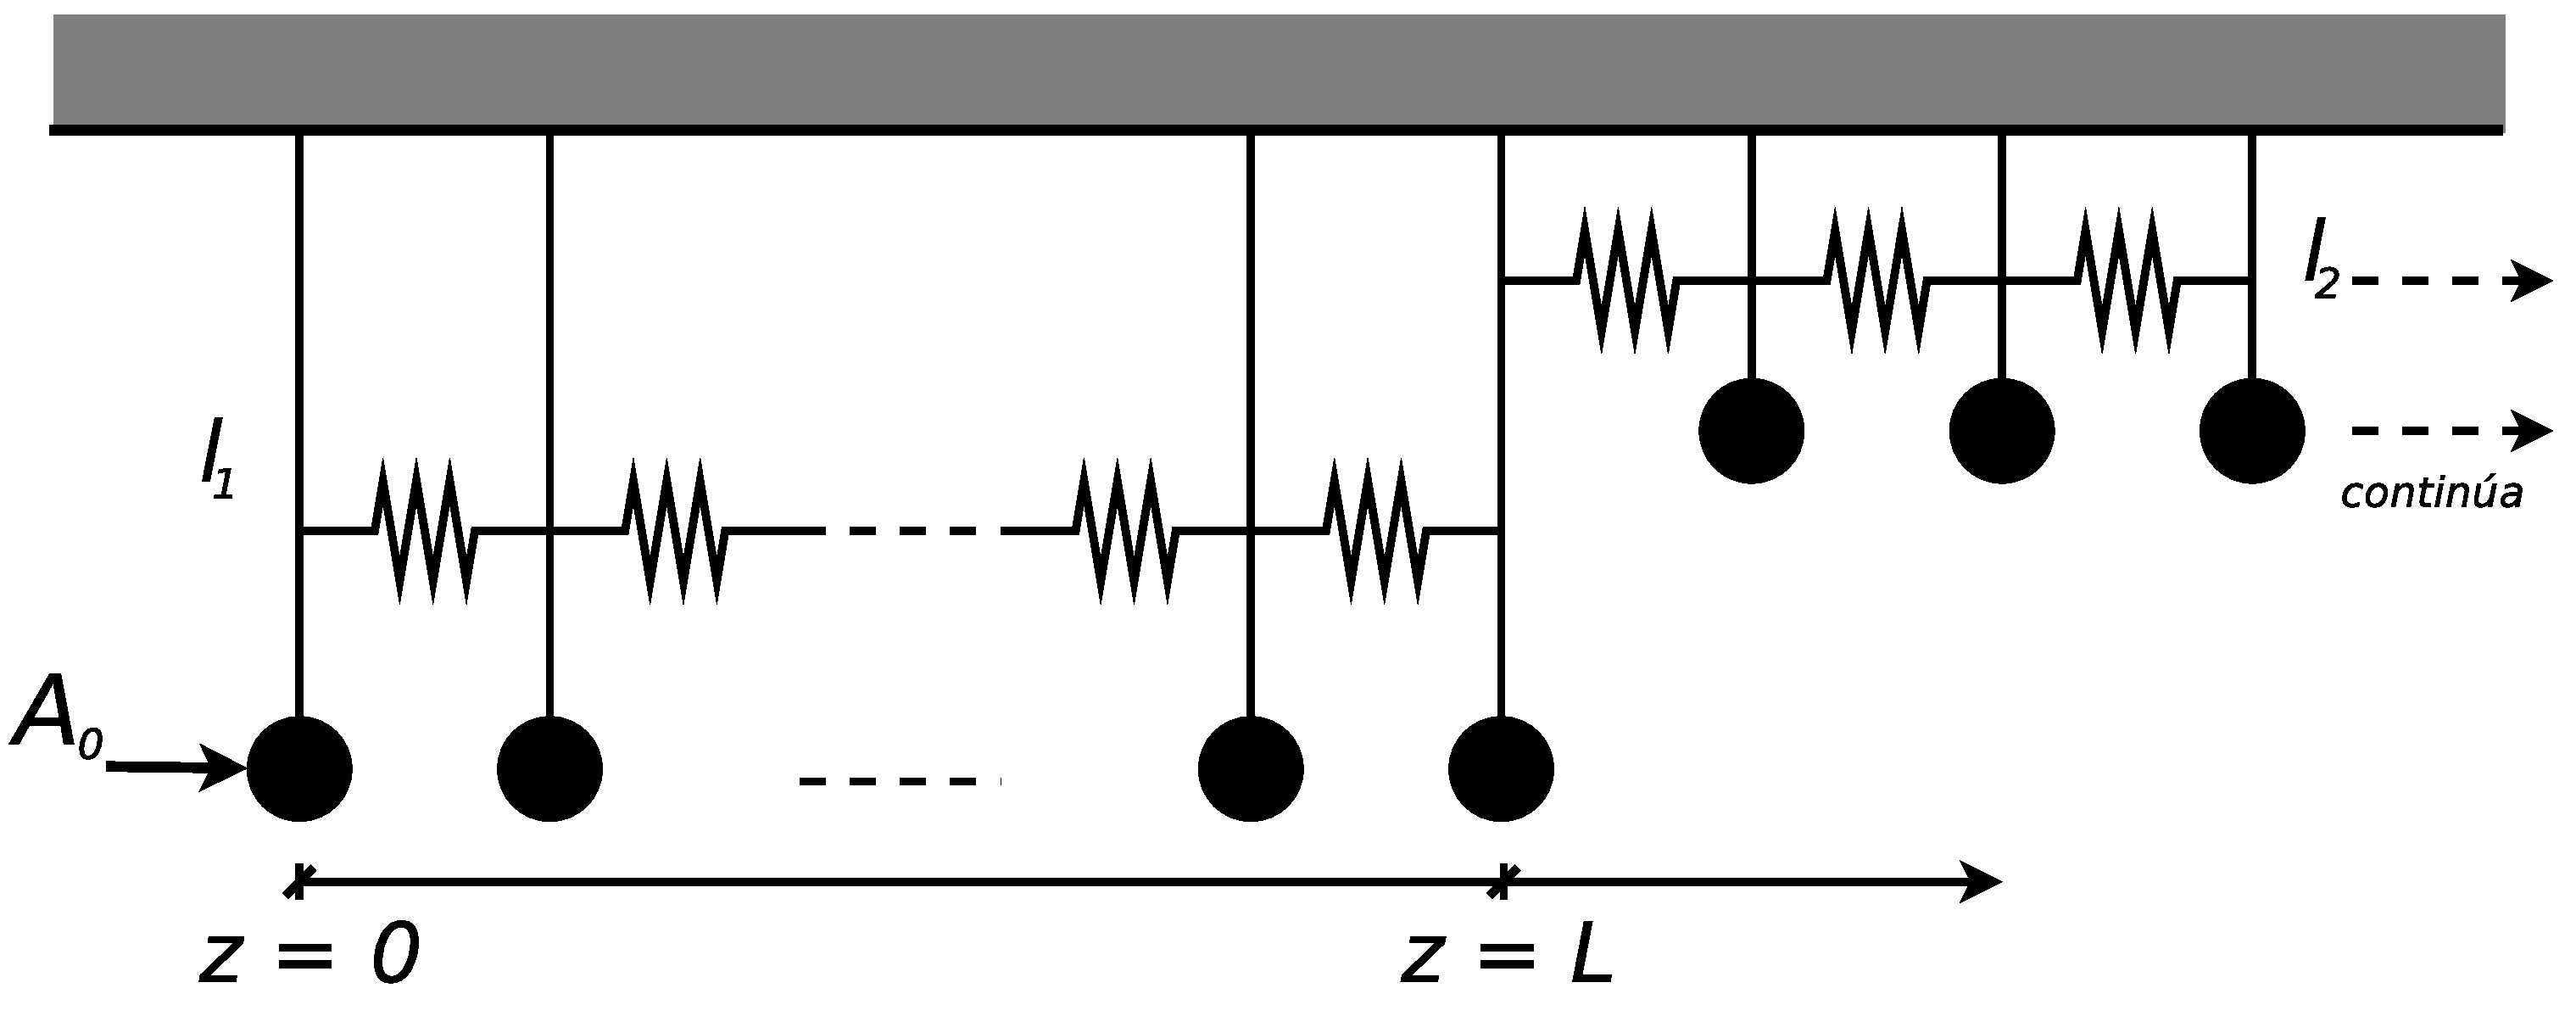
\includegraphics[clip,scale=0.25]{figs/ej1-16}
    \end{figure}

% Ejercicio 10
    
    \item Para el sistema esquematizado en la figura, calcule $\psi_{n}(t)$, si
    $\Omega<\omega_\text{mín}$.

    \begin{figure}[H]
        \centering{}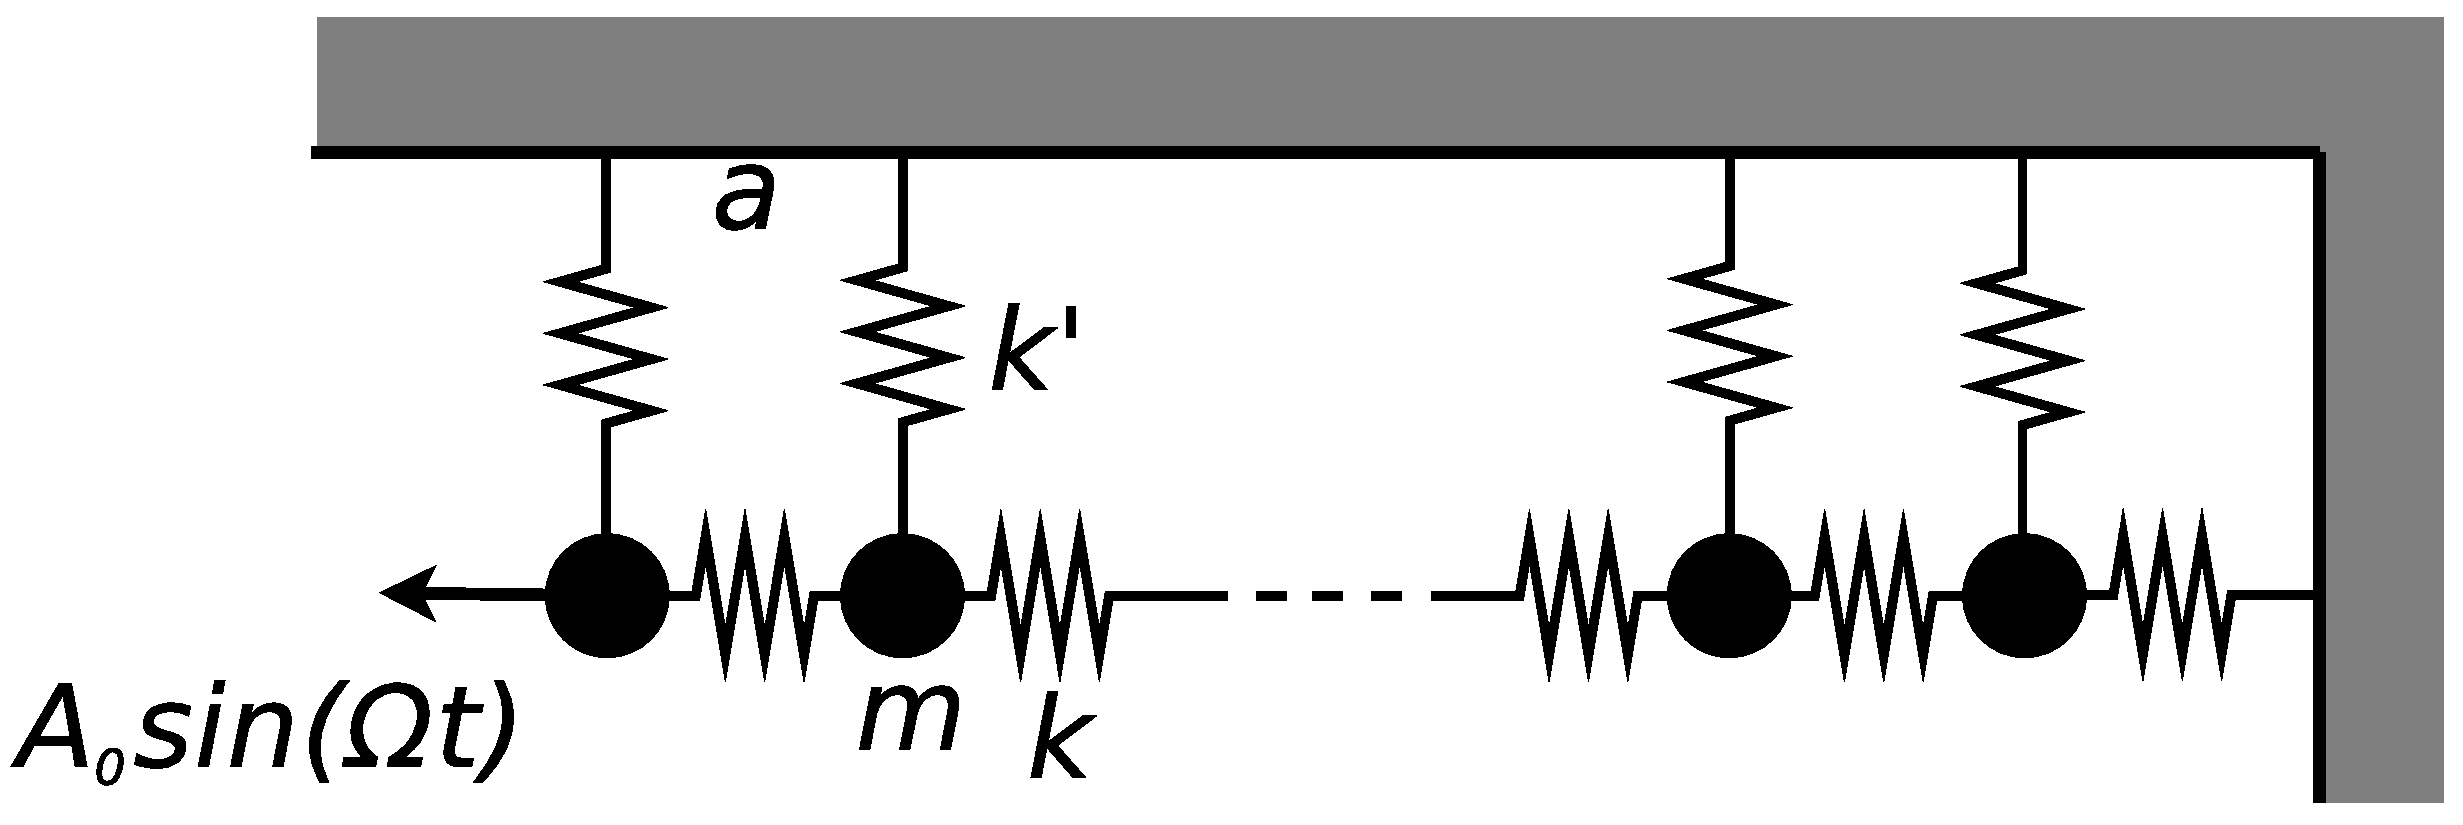
\includegraphics[clip,scale=0.25]{figs/ej1-17}
    \end{figure}

\end{enumerate}

\end{document}

